\documentclass[10pt,a4paper]{article}

%double si on veut une version prof et une version élève. simple si on veut une seule version.
\newcommand{\buildmode}{double}

\InputIfFileExists{version.tex}{}{}
% Version (définie par le script)
\providecommand{\version}{eleve}

\usepackage{feuilleexo}

%%%à modifier à chaque fois

\renewcommand{\niveau}{2nde}
\renewcommand{\chapitre}{Proportions, pourcentages}
\renewcommand{\numchap}{0.2} 
\renewcommand{\theme}{Statistiques}

\begin{document}


%\legendeicones

\vspace{-0.7cm}\begin{prerequis}
\begin{itemize}
    \item Savoir reconnaître et utiliser un tableau de proportionnalité
    \item Savoir effectuer mentalement des multiplications et des divisions avec des petits nombres entiers
\end{itemize}
\end{prerequis}

\prof{
    Au début du cours, bien rappeler ce qu'est une proportion, un sous-effectif et un effectif total. Rappeler les différentes formes que peuvent prendre une proportion.

    Pour cela , on motive l'introduction de ces notions par la volonté de comparer des effectifs de populations différentes. Exemple nombre de panier réussi sur le nombre de panier tenté pour un joueur de basket. On aimerait savoir pendant quel entrainement le joueur à été le plus adroit.
    On utilise les tableau de proportionnalité pour mettre les proportions sous forme de pourcentage. 
    
    Rappeler les fractions remarquables. Faire le lien avec la proportionnalité. Inventer des exos simples (par exemple, avec un tableau de proportionnalité, retrouver les pourcentages correspondants à \(\frac{2}{5}\), \(\frac{3}{5}\)), etc.
    Faire un exemple détaillé et le laisser au tableau pendant qu'ils travaillent.
}

\begin{multicols}{2}
\section{Sans calculatrice}

\vspace{-0.5cm}\begin{exo}[][]

   
    \begin{tasks}(2)
        \task   \renewcommand{\arraystretch}{1.5}  \begin{tabular}{|*{3}{c|}}
        \hline
          9 & 18 & \\ \hline
         25 &  & 100 \\ \hline
    \end{tabular} 

    \task \renewcommand{\arraystretch}{1.5} \begin{tabular}{|*{3}{c|}}
        \hline
          6 & 2 &  \\ \hline
          15 & 5 & 100\\ \hline
    \end{tabular} 
    \end{tasks} 
   


\end{exo}

\prof{
    \begin{enumerate}
        \item Question à poser aux élèves : Comparer \(\frac{6}{15}\) et \(\frac{9}{25}\).
        \item Écrire ces fractions sous forme de pourcentage et sous forme décimale.
    \end{enumerate}
}

\begin{exo}[][appro]
    Les valeurs suivantes sont-elles proportionnelles ? Si oui, complétez les tableaux.
    \begin{tasks}
        \task     \begin{tabular}{|p{4.5cm}|*{3}{c|}}
        \hline
        Distance sur une carte (en cm) & 5 & 7 & \\ \hline
        Distance en réalité (en km) & 10 &  & 20 \\ \hline
    \end{tabular}

    \task     \begin{tabular}{|p{4.5cm}|*{3}{c|}}
        \hline
        Âge (en années) & 1 & 5 & 15 \\ \hline
        Taille (en cm) & 75 &  &  \\ \hline
    \end{tabular}

    \task     \begin{tabular}{|p{4.5cm}|*{3}{c|}}
        \hline
        Nombre de places de cinéma (avec abonnement) & 0 & 3  &  \\ \hline
        Prix total (en euros) & 10 &  & 20 \\ \hline
    \end{tabular}
    \end{tasks}
\end{exo}

\begin{exo}[][]
Calculer :\begin{tasks}(2)
    \task 50\% de 300
    \task 10\% de 45
    \task 25\% de 45
    \task 20\% de 35\%
    \task 75\% de 24\euro
    \task Le quart de 50
    \task le tiers de 10
    \task La moitié de 13,5
\end{tasks}
\end{exo}

\begin{exo}[][]
Dans chacun des cas suivants, calculer la proportion et l'écrire sous forme de fraction, de nombre décimal et de pourcentage.
\begin{enumerate}
    \item Dans une classe de 25 élèves, 4 sont des gauchers.
    \item Dans un collège, 50 élèves sur 500 sont demi-pensionnaires.
    \item Dans un lycée de 100 professeurs, 9 sont professeurs de mathématiques.
\end{enumerate}
\end{exo}

\begin{exo}[][]
La saison 2022-2023 de la ligue 1 de football comptait 65\% d'entraîneurs français.
\begin{enumerate}
    \item Au total, la ligue 1 comptait 20 entraîneurs. Combien d'entraîneurs français y avait-il ?
    \item S'il y avait 60 entraîneurs au total, combien d'entraîneurs français y aurait-il ?
    \item Combien d'entraîneurs y aurait-il si la ligue 1 comptait 130 entraîneurs français  ?
\end{enumerate} 

\textit{Vous avez le droit d'utiliser un tableau de proportionnalité pour vous aider}
\end{exo}
\prof{
    Possibilité d'enlever la question 3c pour la faire à l'oral. À l'oral, faire le lien avec les élèves entre les lignes et les effectifs.\\
    À l'aide du tableau de proportionnalité, rappeler la méthode pour calculer un sous-effectif et un effecif total.
}

\begin{exo}[QCM][]
    
Pour chacune des questions de ce questionnaire à choix multiples, une seule réponse est exacte.

\medskip

\begin{enumerate}[leftmargin=*]
    \item Parmi les 1057 élèves du lycée GT, 333 sont en seconde. Quel est le pourcentage d'élèves en seconde ?
    \begin{tasks}(3)
        \task $10,3\%$
        \task $31,5\%$
        \task $49,1\%$
    \end{tasks}

    \item En 2015, la ville de Saint-Denis comptait 111 103 habitants, parmi lesquels $51,86\%$ environ vivaient dans les quartiers \og La Plaine \fg{}, \og Grand centre-ville \fg{} et \og Franc-Moisin - Bel Air - Stade de France \fg{}. Quel est le nombre d'habitants qui vivaient dans ces quartiers en 2015 ? (Source : \textit{INSEE})
    \begin{tasks}(3)
        \task 26 343
        \task 52 503
        \task 57 615
    \end{tasks}
    \item Lors d'une élection, le quart des électeurs a voté pour le candidat A, \(\frac{1}{5}\) a voté pour B, 34\% a voté pour C et le reste a voté pour D. Le candidat qui a eu le \underline{moins} de voix est :\begin{tasks}(4)
        \task A
        \task B
        \task C
        \task D
    \end{tasks}
\end{enumerate}
\end{exo}
\prof{
    Pour la correction de la question 2, tracer un tableau de proportionnalité.
}

\section{Avec calculatrice}

\vspace{-0.5cm}\begin{exo}[][]
    Sarah, joueuse de basket professionnelle, s'entraîne tous les jours au lanncer franc. Quel jour a-t-elle été le plus habile ? Et le moins habile ?

    \resizebox{0.4\textwidth}{!}{
    \begin{tabular}{|p{1.1cm}|*{5}{c|}}
        \hline
            & Lundi & Mardi &Mercredi & Jeudi & Vendredi \\ \hline
         Paniers tentés & 63 & 46 & 46 & 73 & 53 \\ \hline
         Paniers réussis & 41 & 35 & 31 & 50 & 41 \\ \hline
    \end{tabular}
    }
\end{exo}

\prof{
    \begin{enumerate}
        \item Les nombres 41 et 46 apparaissent deux fois dans le tableau. Cela nous permet de faire une remarque que dans ces cas la comparaison des deux fractions est évidente.

    \end{enumerate}
}

\begin{exo}
    Sur le site de l'académie de Créteil, on peut retrouver les informations suivantes :

    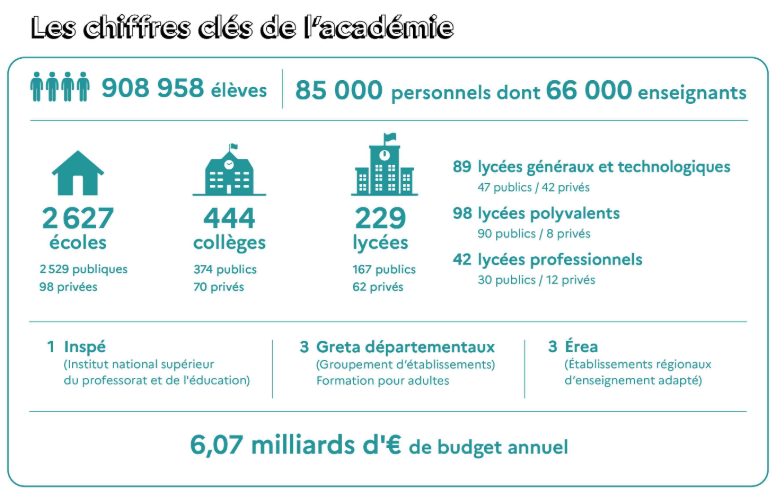
\includegraphics[width=0.45\textwidth]{chiffres_cles_ac_creteil.png}

    \begin{enumerate}
        \item Quelle est la proportion de lycées publiques parmi tous les lycées de l'académie ?
        \item Quelle proportion représentent les enseignants parmi tous les usagers de l'académie ?
        \item En 2026, le budget consacré au ministère de l'éducation nationale est de 85,85 milliards d'euros. Cela représente 10,3\% du budget de l'Etat. Quel est le budget de l'Etat en 2026 ?
    \end{enumerate}
\end{exo}


\end{multicols}
\end{document}
